% !TEX root = ../presentation.tex

% results from 2015 AAS
\subsubsection[PRCTBP]{Three Body Problem}

\begin{frame}%--------------------------------------------%
\frametitle{Three Body Problem}
    \begin{itemize}
        \item Transfer from \( L_1 \) orbit to periodic orbit near the Moon
        \item Bounded control input and fixed time horizon
    \end{itemize}
    \visible<2>{
        \begin{center}
            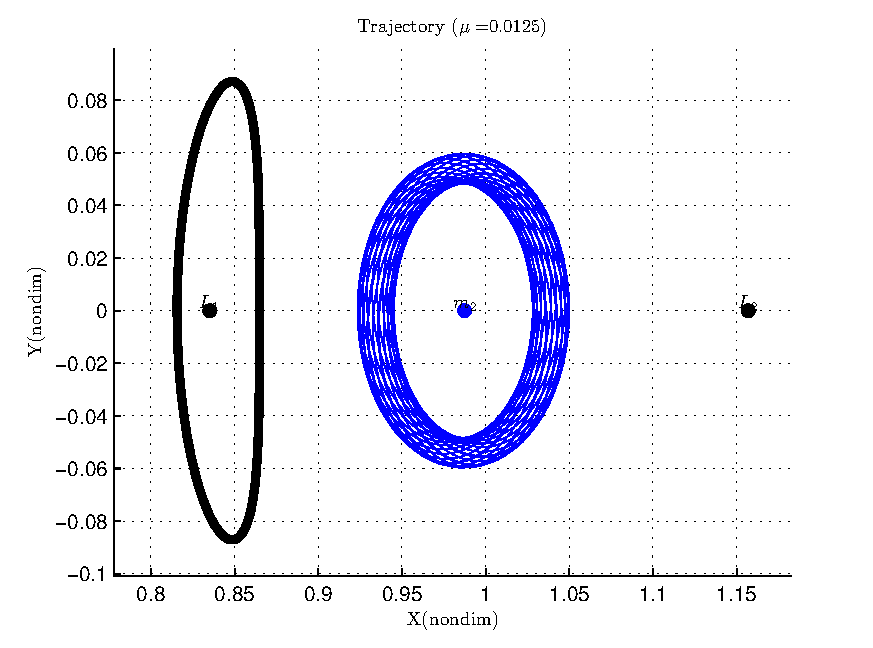
\includegraphics[width=0.7\textwidth,height=0.7\textheight,keepaspectratio]{2015AAS/moon_orbit.pdf}
        \end{center}
        }
    
    \note[itemize]{
        \item Introduce problem and initial and terminal orbits. 
        \item Earth is way off to the left with the Moon at the center
        \item Possible use as a communication array
        \item Might actually be a distant retrograde orbit
        }
\end{frame} %--------------------------------------------%

\begin{frame}%------------------------------------------------%
    \frametitle{Reachable Set Transfer}
    \begin{itemize}
        \item Approximate the reachable set on the \Poincare section
        \begin{itemize}
            \item Generate many optimal solutions
        \end{itemize}
        \item<3-> Intersection point used to generate a transfer
        \begin{itemize}
            \item Shorter time of flight than uncontrolled dynamics
        \end{itemize}
    \end{itemize}
    \begin{center}
        \only<1-2>{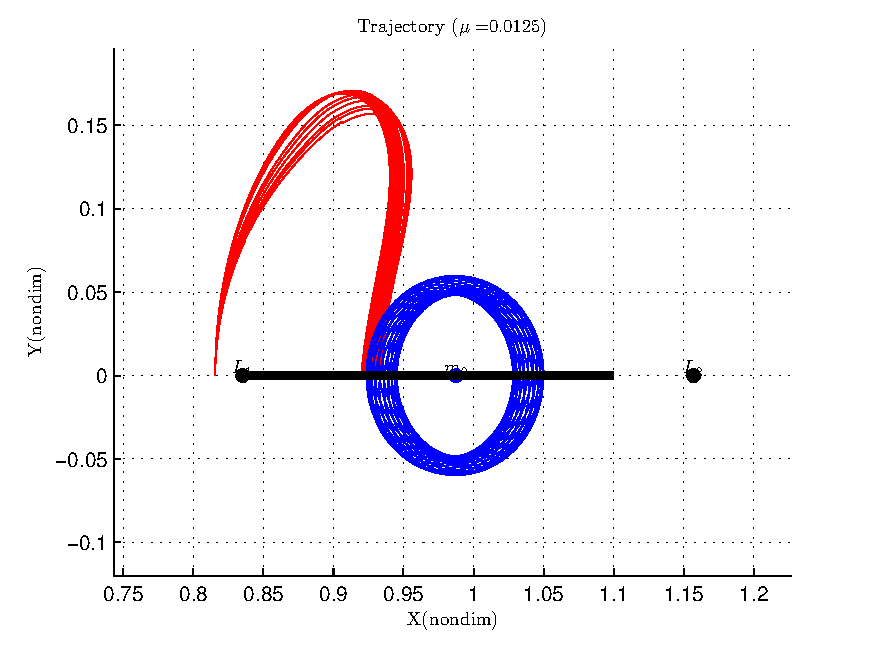
\includegraphics[width=0.5\textwidth,height=0.7\textheight,keepaspectratio]{2015AAS/reach_trajectory}~}
        \only<3->{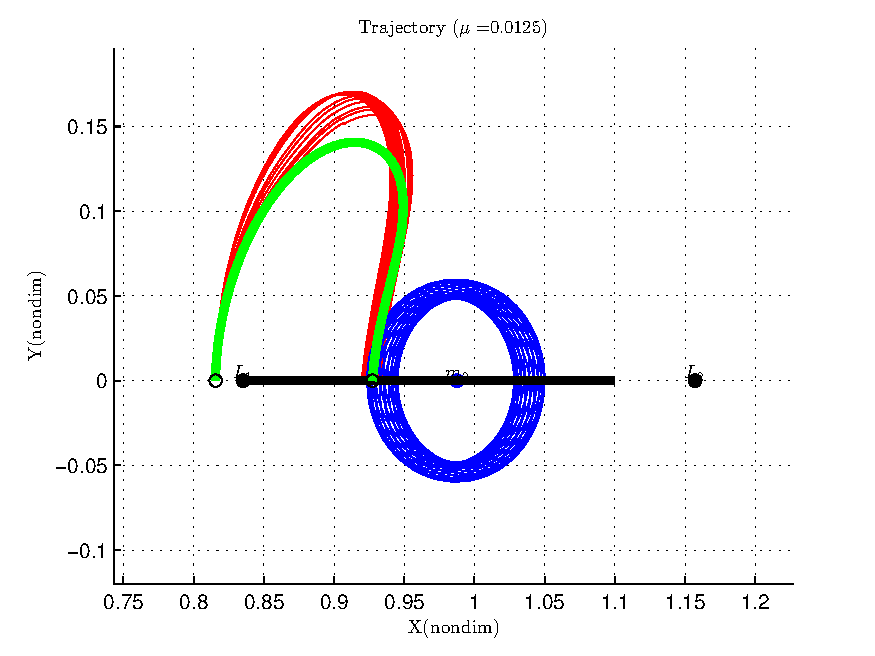
\includegraphics[width=0.5\textwidth,height=0.7\textheight,keepaspectratio]{2015AAS/reach_transfer}~}
        \only<2-3>{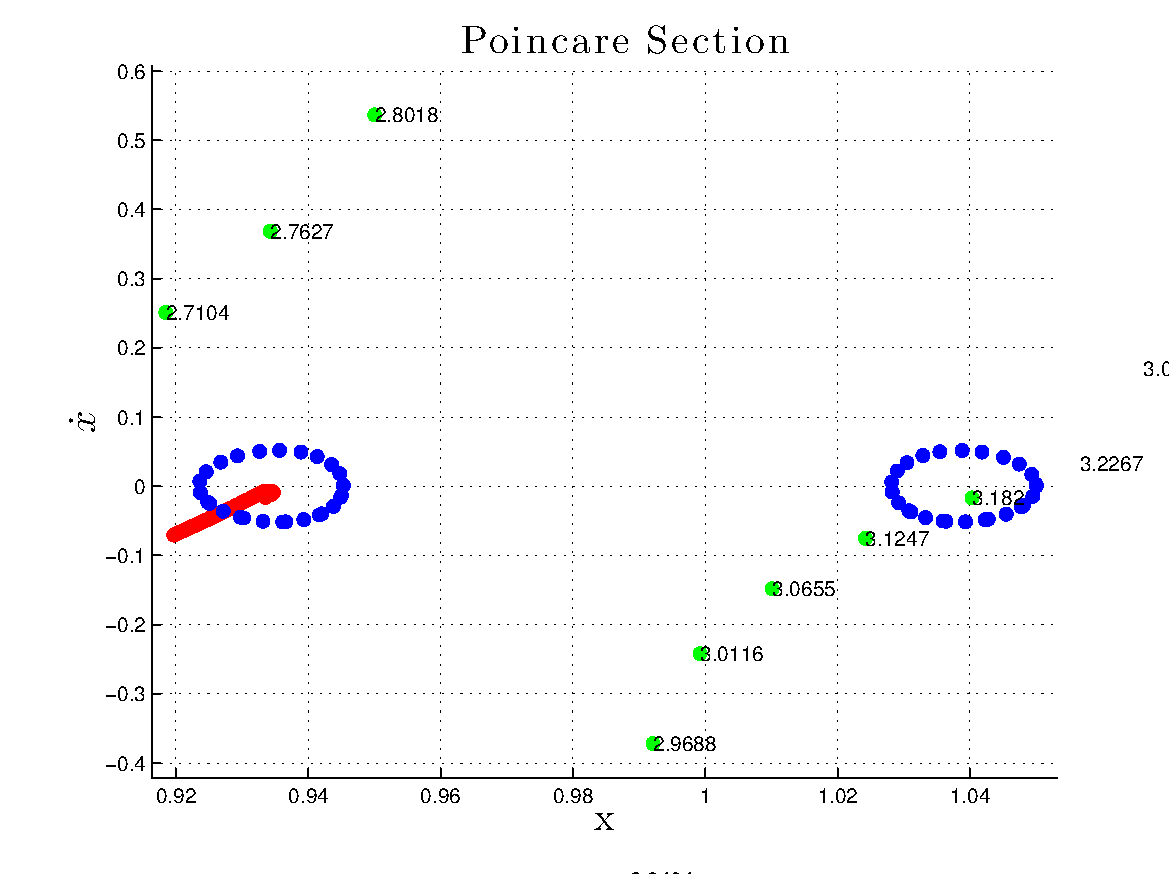
\includegraphics[width=0.5\textwidth,height=0.7\textheight,keepaspectratio]{2015AAS/poincare_compare}} 
    \end{center}
    
    \note[itemize]{
        \item Compare to reachable set approach
        \item Shorter time of flight
        \item Multiple shooting to solve TPBVP
        Vary \( \theta\) to change direction on section
        Linear interpolation to determine intersection on Poincar\'e section
        \item Only one reachabile set computation is required
        }
\end{frame} %--------------------------------------------------%

\begin{frame}{Geostationary  transfer} %----------------------------------------------------%
    \begin{itemize}
           \item Transfer from geostationary orbit to a \( L_1\) periodic orbit 
           \item Multiple iterations of reachable set required for transfer
    \end{itemize}

    \begin{center}
       \only<1>{
       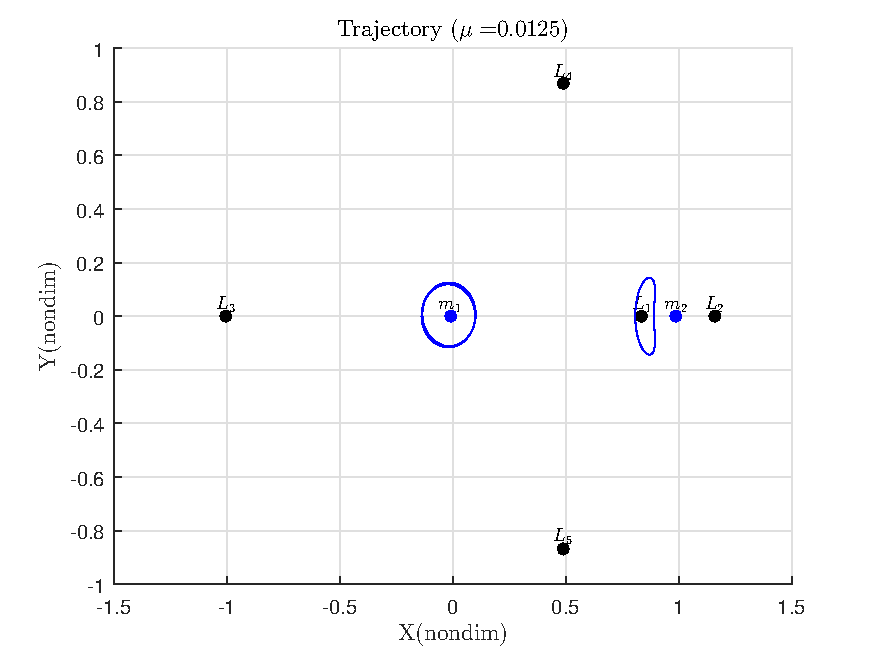
\includegraphics[width=0.5\textwidth,height=0.7\textheight,keepaspectratio]{figures/2015ACTA/initial_final.pdf}~
       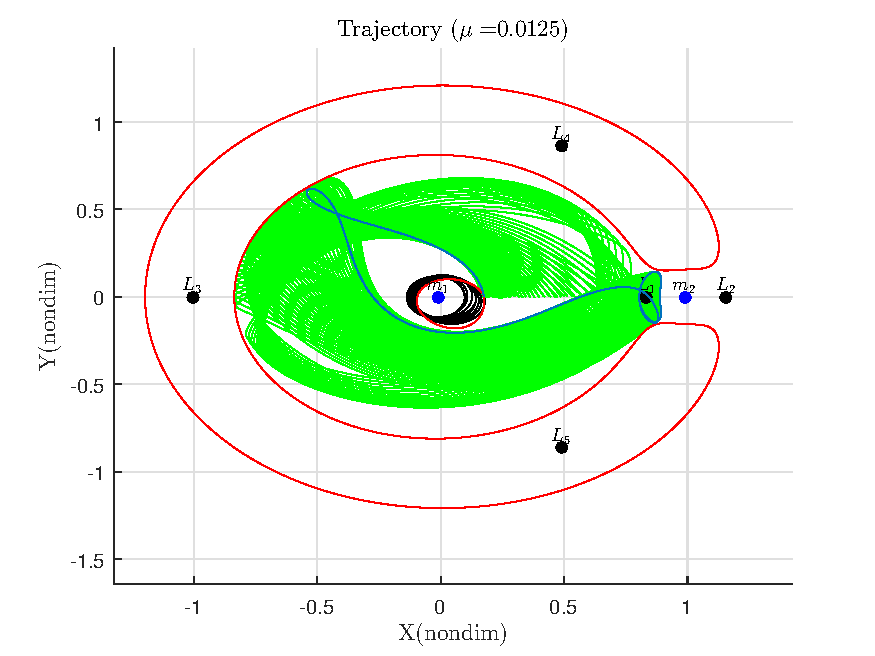
\includegraphics[width=0.5\textwidth,height=0.7\textheight,keepaspectratio]{figures/2015ACTA/geo_transfer_full.pdf} 
       }

       \only<2>{
       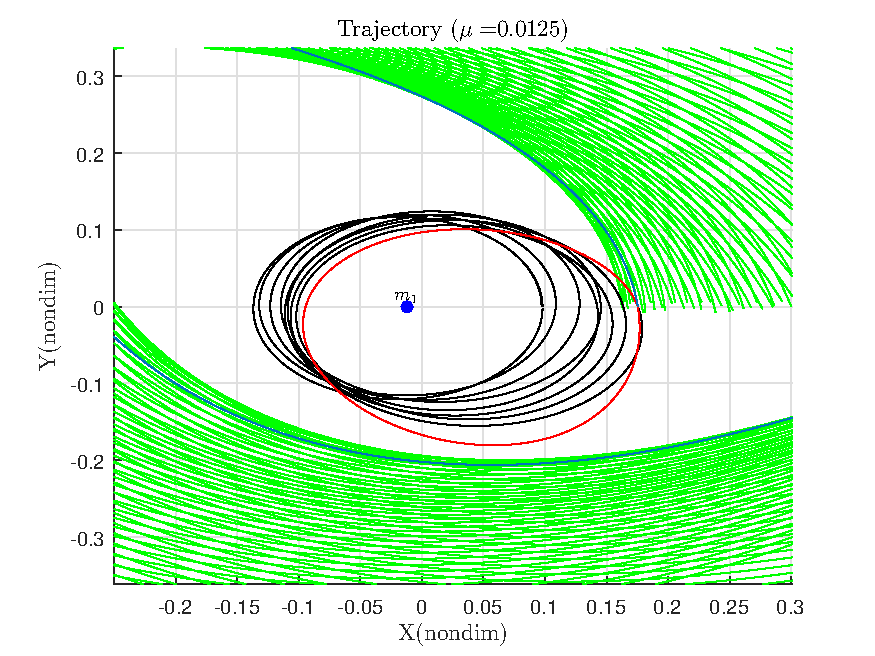
\includegraphics[width=0.5\textwidth,height=0.7\textheight,keepaspectratio]{figures/2015ACTA/geo_transfer_zoom.pdf}~
       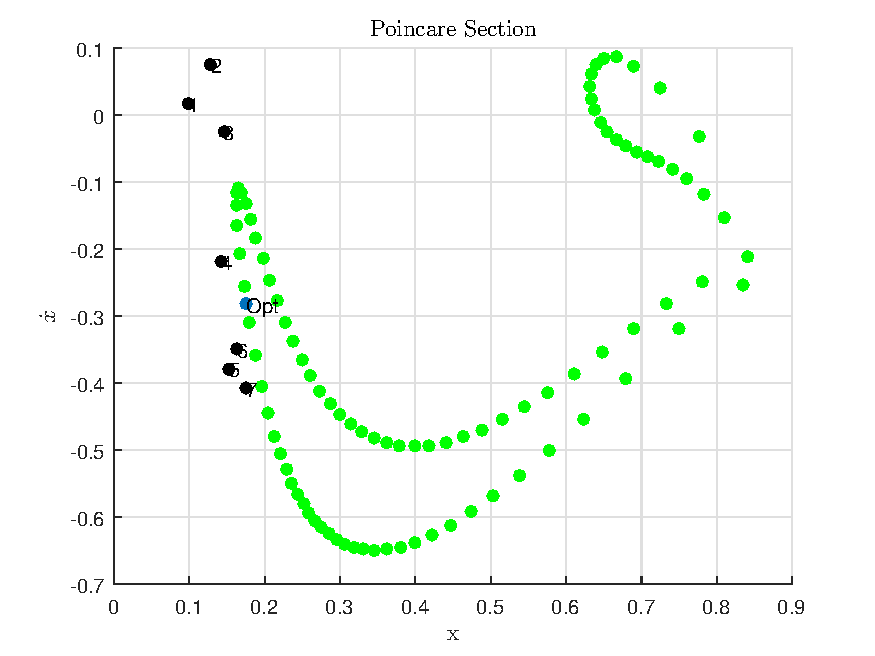
\includegraphics[width=0.5\textwidth,height=0.7\textheight,keepaspectratio]{figures/2015ACTA/poincare.pdf}
       }
    \end{center}

\note[itemize]{
    \item The green trajectories are the invariant manifolds and require no control input to traverse large regions of the phase space
}
\end{frame} %--------------------------------------------%
